%Linea Para poder completar automaticamente las citas con el Sublime
%No hace el documento, se puede borrar esta linea si no se usa el Sublime
%------------------------------------------------------------------------------
 \newcommand{\NoBiblioMat}[1]{
 \ifthenelse{\equal{#1}{verdadero}}{}{\bibliography{Referencias/base_bibliografica}}
 \NoBiblioMat{verdadero}}
 %-----------------------------------------------------------------------------

%Formato (Nombre de capitulo largo o corto), nombre del capitulo y estilo de la
%Portada del Capitulo
%------------------------------------------------------------------------------

 %Formato en si, titulo en un solo renglon
 \FormatoCapituloUnaLinea

 %Nombre y etiquete para referir
 \chapter{Materiales, Métodos y Procesos}\label{chap:Materiales}

 %Para que no salga el numero de pagina en la portada del capitulo
 \thispagestyle{empty}
	
 %Resumen del Capitulo en Italica 
  \noindent\textit{En este capitulo se presenta la descripción experimental de todos los materiales, instrumental y procesos involucrados en la tesis. En la primera sección se detallan los procesos de síntesis de las películas mesoporosas, desde la preparación de los soles hasta la caracterización de las mismas; en la segunda se presentan los procesos de fabricación de los electrodos, desde el diseño a las técnicas de transferencia; la tercera sección describe las técnicas de microscopías utilizadas y la última sección detalla como se llevaron a cabo las mediciones electroquímicas.}


 %Indice de capitulo alineada al borde inferior de la pagina, nueva pagina
 \vfill
 \minitoc
 \newpage

 %-------------------------------------------------------------------------------

\section{Síntesis de películas delgadas mesoporosas}\label{sec:sintesis_mesoporosos}	
	
	 Las consideraciones teóricas sobre la química sol-gel y el autoensamblado inducido por evaporación (AEIE) ya fueron expuestas en el capítulo \ref{chap:Introduccion}. También fueron mencionadas las razones por las cuales se eligió SiO$_2$ como estructura para las películas delgadas mesoporosas y Pluronic F127 o CTAB como agente moldeante. Los procedimientos, métodos y proporciones molares para la preparación de los soles fueron, en su mayoría, adaptaciones de los trabajos de Angelomé\cite{Angelome2008} y Fuertes\cite{Fuertes2009}. El esquema \ref{esq:peliculas_meso} resume cada etapa de síntesis de las películas, que se explican con detalle en las próximas secciones.
		  \begin{figure}[ht]
			  \begin{center}
			  \includegraphics[width=\textwidth]{Esquemas/Resumen_sintesis_meso.pdf}
			  \caption[Síntesis de películas delgadas mesoporosas]{Diagrama de flujo para la síntesis de películas delgadas mesoporosas.}
			  \label{esq:peliculas_meso}
			  \end{center}
			  \end{figure}
			  \vspace*{-0.2cm}

	\subsection{Preparación de los soles, reactivos y nomenclatura}\label{sec:soles}
		
			La síntesis y depósito de las películas delgadas mesoporosas comienzan con la preparación de las soluciones, las cuales deben contener los precursores del óxido (o de los óxidos en el caso de películas mixtas), el agente moldeante de los poros, solvente adecuado, H$_2$O y HCl\cite{Brinker1990}. Cada uno de estos componentes cumple una función especifica, tal como se explicó en la sección \ref{sec:mesoporosos}. Los precursores utlizados fueron tetraetoxisilano (TEOS, \textit{Merck}) para las películas de sílice pura, y TEOS combinado con cloruro de circonio(IV) (ZrCl$_4$, \textit{Aldrich}) para las películas mixtas de silicio/circonio. Las condiciones de hidrólisis y condensación para estos dos reactivos (ya sean solos o combinados) son bien conocidas y llevan a la formación películas delgadas estables y reproducibles de óxidos mesoporosos puros o mixtos\cite{Soler-Illia2004,Crepaldi2002a,Angelome2008}. El surfactante es el agente que establece el tamaño de los poros, se utilizó para ello el copolímero de bloque Pluronic F127 (F127, \textit{Aldrich}) y bromuro de hexadeciltrimetilamonio (CTAB, \textit{Aldrich}). Como solvente se utilizó etanol absoluto (EtOH, \textit{Sigma}). El H$_2$O es el reactivo para la formación del óxido mediante la conexión de los grupos metálicos M(IV). Por último, el HCl es el encargado de generar el medio ácido que cataliza la hidrólisis y controla la condensación del Si(IV) y/o del Zr(IV). Los reactivos utilizados fueron de calidad proanalisis o superior y el H$_2$O de \SI{18}{\mega\ohm\per\cm} fue obtenida con un equipo \textit{Ultra Clear TWF} de la marca \textit{Siemens}. La nomenclatura, pesos moleculares y estructura química de los reactivos utilizados se pueden consultar en la tabla \ref{tabla:reactivos}.
					
			El preparado de las soluciones se realizó agregando cada reactivo por pesada en balanza analítica. Cada lote de solución fue de aproximadamente \SI{100}{\ml}. Para llegar a este volumen se agregaron, en este orden, \SI{10.417}{\gram} de TEOS, \SI{6.911}{\gram} de etanol y \SI{0.902}{\gram} de HCl \SI{2,77e-3}{\Molar}. En el caso de los soles mixtos (Si/Zr 9:1), se pesaron \SI{9.375}{\gram} de TEOS y \SI{1.165}{\gram} de ZrCl$_4$. Esta primera solución, denominada solución de prehidrólisis, se deja envejecer bajo agitación constante durante \SI{48}{\hour} a \SI{25}{\celsius}, con el objetivo de hidrolizar los precursores metálicos y mantener un bajo grado de condensación.\cite{Grosso2001}

				\begin{table}[ht!] 
						  \caption[Reactivos para los soles]{Nomenclatura, estructura, peso molecular y función de las moléculas utilizadas en las soluciones para la síntesis de películas delgadas mesoporosas.} 
				  		  \begin{tabular}{>{\raggedright\arraybackslash}m{2.40cm}>{\centering\arraybackslash}m{4cm}>{\centering\arraybackslash}m{2.35cm}>{\raggedright\arraybackslash}m{1.7cm}} 
				  		  \toprule
						  Nombre Nomenclatura    & Estructura & Peso molecular \si{g.mol^{-1}} & Función\\ \midrule
				      	  tetraetoxisilano TEOS & \includegraphics[scale=0.5]{Esquemas/teos.pdf} & $208,33$ & precursor del óxido  \\ \midrule
				      	  \mbox{cloruro de circonio(IV)}  ZrCl$_4$ & \includegraphics[scale=0.8]{Esquemas/zrcl4.pdf} & $233.04$ & precursor del óxido  \\ \midrule
				  		  Pluronic F127 F127    & \hspace*{-10px} 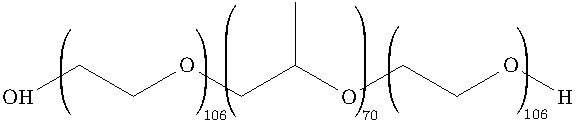
\includegraphics[scale=0.5]{Esquemas/f127.pdf} & \multirow{1}{*}{$13800$}	 & agente moldeante	 \\ \midrule
				  		  bromuro de hexadeciltrimetilamonio  CTAB   & \hspace*{1cm} 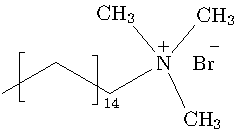
\includegraphics[scale=0.6]{Esquemas/ctab.pdf} & \multirow{1}{*}{$364.48$}	 & agente moldeante	 \\ \midrule
				  		  ácido clohídrico HCl& \includegraphics[scale=0.75]{Esquemas/hcl.pdf}  & \multirow{1}{*}{$36,46$}   & cataliza la hidrólisis \\ \midrule
				  		  agua \hspace{2cm} H$_2$O  &  \includegraphics[scale=0.75]{Esquemas/agua.pdf}  & \multirow{1}{*}{$18,02$}   & reactivo de hidrólisis \\ \midrule
				  		  etanol \hspace{2cm} EtOH  & \includegraphics[scale=0.75]{Esquemas/etanol.pdf}  & \multirow{1}{*}{$46,07$}   & solvente \\ 
				  		  \bottomrule
				    	  \end{tabular}
				   		  \label{tabla:reactivos}
					      \end{table}

			Una vez envejecida la solución de prehidrólisis (ya sea de SiO$_2$ pura o mixta) se agregan a \SI{17.146}{\gram} de esta, \SI{80.184}{\gram} de EtOH, \SI{3.246}{\gram} de F127 o \SI{1.822}{\gram} de CTAB y \SI{7.630}{\gram} de HCl \SI{2,5e-2}{\Molar}. De esta forma se obtienen unos \SI{100}{\ml} de un sol con las relaciones molares de la tabla \ref{tabla:soles}. Se conservan en \textit{frezeer} a \SI{-18}{\celsius} y sólo se retiran a la hora de depositar las películas. 

			Para facilitar la lectura se utilizará la siguiente nomenclatura, tanto para los soles como para las películas delgadas mesoporosas que se fabriquen con ellos: 

				\begin{itemize}
			 			\item \pdm\space para películas delgadas mesoporosas en general.
			 			\item \pdmF\space para \pdm\space de óxido de silicio estructuradas con F127. 
			 			\item \pdmC\space para \pdm\space de óxido de silicio estructuradas con CTAB.
			 			\item \pdmZ\space para las \pdm\space mixtas de óxido de circonio y silicio en relación molar $1\!:\!9$ y estructuradas con F127. 
					    \end{itemize}	
			
			Todas las soluciones fueron preparadas indistintamente en el Centro de Micro y Nanoelectrónica del Bicentenario del Instituto Nacional de Tecnología Industrial (INTI-CMNB) o en la Gerencia Química, Centro Atómico Constituyentes Comisión Nacional de Energía Atómica (CAC-CNEA). 
					
				\begin{table}[h!]
			  		  \caption[Relación molares de los soles]{Relaciones molares para las soluciones utilizadas.} 
			  		  \begin{tabular}{>{\raggedright\arraybackslash}m{2.2cm}>{\centering\arraybackslash}m{2.2cm}>{\centering\arraybackslash}m{1.875cm}>{\centering\arraybackslash}m{1.875cm}>{\centering\arraybackslash}m{1.875cm}} 
			  		  \toprule
					  Componente & Prehidrólisis  & \pdmF   & \pdmC  & \pdmZ \\  \midrule
			      	  TEOS 		  & 1/0,9$^*$	  & 1   	& 1		 & 0,9   \\ \midrule
			      	  ZrCl$_4$	  & -/0,1$^*$	  &	-		& - 	 & 0,1   \\ \midrule	
			      	  EtOH 		  & 3			  & 40   	& 40	 & 40    \\ \midrule
			      	  F127 		  & -		 	  & 0,0075  & -		 & 0,0075\\ \midrule
			      	  CTAB 		  & -             & -		& 0,1	 & 0,1   \\ \midrule
			      	  H$_2$O	  & 1			  & 9	  	& 9	     & 9     \\ \midrule
			      	  HCl    	  & 0,00005		  & 0,01   	& 0,01	 & 0,01   \\ 
			      	  \bottomrule
			    	  \end{tabular}\vspace*{2pt}
		    	  	  \footnotesize{$^*$Los números después de la barra son los utilizados en soluciones de prehidrolisis para películas mixtas de silicio/circonio.}
			    	  \label{tabla:soles}
			   		  \end{table}

	\subsection{Depósitos de las películas delgadas mesoporosas}\label{sec:deposito_pdm}

			Las películas mesoporosas utilizadas en esta tesis fueron depositadas en el Laboratorio de Fotolitografía del INTI-CMNB por \textit{spin-coating}. La técnica consiste en un portamuestras acoplado a un cabezal rotatorio que al girar dispersa el líquido para formar una película sobre el sustrato.

			Como sustrato para realizar los depósitos se utilizaron: vidrio, silicio, oro sobre silicio, microelectrodos y sustratos poliméricos como  polimetilmetacrilato (PMMA) y poliestireno de alto impacto (PAI). Cada uno de ellos fue escogido para una función particular (p. ej. sustrato para reacciones electroquímicas) o por alguna característica distintiva (p. ej. transparente en el IR). En la tabla \ref{tabla:sustratos}, pág. \pageref{tabla:sustratos}, se agrupan los sustratos utilizados y se resumen algunas características y funciones destacadas.

			Las dimensiones de las muestras fueron típicamente de \SI{1x1}{\cm} a \linebreak \SI{2x2}{\cm}, aunque la técnica permite depositar películas continuas de hasta \SI{15}{cm} de diámetro. En algunos casos, para obtener lotes de 32 o 46 sensores (dependiendo del diseño), se utilizaron obleas de silicio de \SI{10}{\cm} de diámetro. Antes de hacer el depósito, el sol se pasa a través de un filtro de jeringa de nailon de \SI{0.45}{\um} (\textit{GAMAFIL}) para evitar la presencia de partículas que puedan generar discontinuidades y/o <<cometas>> en los depósitos\cite{Franssila2004}. Luego, para dispensar el sol en el sustrato, se utilizaron pipetas tipo Pasteur o pipetas automáticas dependiendo del volumen requerido, el cual varió de 80 a \SI{100}{\uL.\cm^{-2}}. Las condiciones del laboratorio durante el depósito se mantuvieron en \SI{25}{\celsius} y a una HR entre 30\% y 50\%. Una vez dispensado el sol, se da comienzo a la rotación que dispersa la solución de manera homogénea sobre el sustrato y, a su vez, la evaporación del solvente promueve la formación del cristal líquido por el mecanismo de AEIE\cite{Brinker1999}.


			El espesor de la película, ($t$), es inversamente proporcional a la raíz cuadrada de la velocidad angular ($\omega$), es decir $t\propto \omega ^{-1/2}$. Las rampas de velocidad y aceleración fueron optimizadas para obtener \pdm\space con espesores entre 150 y \SI{300}{\nm}\cite{Meyerhofer1978,Hall1998,Brinker1990}. Los esquemas aplicados se muestran en gráfico de la figura \ref{fig:rampa-spin}. 
				
					
			 	    \begin{table}[ht!]
			  		   \caption[Sustratos utilizados para el depósito de \pdm]{Sustratos utilizados para el depósito de \pdm.} 
			  		   \begin{tabular}{>{\raggedright\arraybackslash}m{2.4cm}>{\raggedright\arraybackslash}m{2.5cm}>{\raggedright\arraybackslash}m{2cm}>{\raggedright\arraybackslash}m{3.55cm}} 
			  		   \toprule
					   Sustrato Nomenclatura   & Observaciones  & Limpieza previa$^*$ & Función \\ \midrule
			       	   vidrio \hspace{2cm} Vi  &	portaobjetos \textit{BioTraza} & inmersión KOH 40\% & económico para pruebas preliminares de depósito \\ \midrule
			       	   silicio\hspace{2cm} Si  & Si[100] pulido dopado tipo n  \textit{Addison}& inmersión HF 48\% & FTIR, MEB, FIB, PEA \\ \midrule
			       	   Au sobre silicio\hspace{2cm} Si$|$Au & depositado por pulverización catódica$^\dagger$  & ultrasonido en H$_2$O  & transporte, EQ\\ \midrule
			      	   microelectrodos \hspace{2cm} $\mu Elec$ & sensores, diseño transferido por fotolitografía$^\mathsection$  	  &  ultrasonido en H$_2$O  & multisensado, EQ \\ \midrule
			      	   poliméricos         &  PMMA y PAI		  &  ultrasonido en H$_2$O &  demostrador métodos suaves de síntesis\\ 
			      	   \bottomrule
			    	   \end{tabular}\vspace*{2pt}
			    	   \footnotesize{$^*$Ver la sección <<\nameref{sec:limpieza}>>, tabla \ref{tabla:limpieza}, pág. \pageref{sec:limpieza}.}\\
			    	   \footnotesize{$^\dagger$Ver la sección <<\nameref{sec:sputt}>>, pág.\pageref{sec:sputt}.} \\
			    	   \footnotesize{$^\mathsection$Ver la sección <<\nameref{sec:fotolito}>>, pág. \pageref{sec:sputt}.}
			    	   \label{tabla:sustratos}
			   		   \end{table}

			   		   \begin{figure}[!ht]
						 \begin{center}
						 \includegraphics[width=0.70\textwidth]{Graficos/rotacion_meso.pdf}
						 \caption[Parámetros de depósito para las \pdm]{Esquema con las rampas más frecuentes de aceleración, velocidad y tiempo utilizadas para el depósito de \pdm.}
						 \label{fig:rampa-spin}
						 \end{center}
						 \end{figure}
			
			 El equipo utilizado fue un \textit{Suss MicroTec Delta 20BM}, el cual consiste en un cabezal rotatorio con control de aceleración (0 a  \SI{1000}{\minute^{-1}.\second^{-1}}) y velocidad angular (0 a \SI{10000}{\minute^{-1}}). Posee múltiples portamuestras para sustratos de diferentes tamaños con entrada de vacío para sujetar las muestras (figura \ref{fig:spin}).   		   

					\begin{figure}[ht!]
					  \begin{center}
					  \includegraphics[width=\textwidth]{Imagenes/Spin.jpg}
					  \caption[Equipo para el depósito de películas delgadas, \textit{spin-coater}]{\textit{Spin-coater} ubicado en el Laboratorio de Fotolitografía del INTI-CMNB utilizado para el depósito de las películas delgadas mesoporosas, Marca \textit{Suss MicroTec}, modelo \textit{Delta 20BM}.}
					  \label{fig:spin}
					  \end{center}
					  \end{figure}

	\subsection{Eliminación del surfactante}\label{sec:cond_y_extr}

		Una vez realizado el depósito, se debe conservar la estructura del cristal líquido obtenido, y evitar el deterioro durante la eliminación del surfactante. Para ello se estabiliza la película durante \SI{1}{\hour} en cámara de humedad controlada a una HR constante de 50\%. Para mantener dicho valor de humedad se utilizó una solución saturada de Ca(NO$_3$)$_2$.5H$_2$O (\textit{Biopack}). Controlar la presión parcial de agua (P$_{\text{H}_2\text{O}}$) permite optimizar el grado de condensación del óxido y ayuda a la separación de fases entre el agente moldeante y el óxido\cite{Crepaldi2003}. El proceso de estabilización y condensación del óxido continua con un calentamiento en plancha calefactora, (\textit{Cimarec}) una hora a \SI{60}{\celsius} y una hora más a \SI{130}{\celsius}\cite{Crepaldi2003,Crepaldi2002a}. 
				
		Posteriormente a la estabilización de la película se experimentaron varios tratamientos para completar el proceso de condensación de la fase inorgánica y extraer el surfactante para dar lugar a la película nanoporosa, a saber:

				\begin{itemize}

				\item \textit{Calcinacion.} Este es el proceso clásico en el cual se somete a la película a una temperatura de \SI{350}{\celsius} durante \SI{2}{\hour} con una rampa de \SI{1}{\celsius.\minute^{-1}} (Horno \textit{Indef 337}). De esta forma se condensa el óxido, se elimina el surfactante y se minimiza el daño de la estructura tridimensional de la red nanoporosa \cite{Crepaldi2003}.

				\item \textit{Condensación ácida.} En este método se busca promover la condensación de la matriz inorgánica mediante la exposición de las películas a una atmósfera de vapores de HCl \cite{Doshi2000a}. El arreglo para tal fin consiste en sujetar las muestras al fondo de un vaso de precipitados y colocarlo invertido sobre un cristalizador con HCl concentrado (\textit{Biopack}) durante \SI{10}{\minute}. 

				\item \textit{Condensación alcalina.} Al igual que el método anterior, se busca promover la condensación del óxido cambiando las condiciones del entorno químico, en este caso someter las películas a una atmósfera de pH alcalino generada con vapores de NH$_3$ (\textit{Biopack}) \cite{Soler-Illia2012,Soler-Illia2011}. El armado experimental fue igual que el descripto para el método ácido.

				\item \textit{Tratamiento a \SI{130}{\celsius}.} Esta estrategia de síntesis involucró dejar las muestras en estufa a \SI{130}{\celsius} durante 7 días con el objetivo de promover la condensación del óxido.

				\item \textit{Alto vacío.} Este tratamiento consiste en dejar las muestras en una cámara de alto vacío a \SI{1e-5}{\milli\bar} y \SI{130}{\celsius} durante 7 días. Para calentar y llegar al vacío necesario se utilizó la cámara de una soldadura de obleas (\textit{EVG 501 Manual Wafer Bonding System}) la cual fue evacuada por una bomba mecánica y una turbomolecular secuencialmente.

				\end{itemize}
					
		En los casos donde fue necesario realizar la extracción del surfactante sin calcinar, las muestras fueron sometidas a un reflujo de isopropanol a punto de ebullición (\textit{Biopack}) durante \SI{15}{\minute}. Luego se enjuagaron con H$_2$O acidificada con HCl a $\text{pH}=2$. El siguiente diagrama de flujo resume y agrupa los tratamientos realizados sobre las \pdm, desde el depósito hasta la extracción del surfactante.
		
				\begin{figure}[ht!]
						  \begin{center}
						  \includegraphics[width=\textwidth]{Esquemas/Resumen_extraccion.pdf}
						  \caption[Tratamientos pos-depósito de \pdm]{Etapas de estabilización y diferentes tratamientos pos-depósito utilizados para condensar las \pdm\space, tanto de óxidos puros como las mixtas y extraer el surfactante.}
						  \label{esq:peliculas_meso_tratamientos}
						  \end{center}
						  \end{figure}

	\pagebreak \subsection{Espectroscopia IR}\label{sec:IR}

		La región infrarroja (IR) del espectro electromagnético puede ser divido en tres zonas, según su longitud de onda, IR cercano (400 a \SI{10}{\cm^{-1}}), IR medio (4000 a \SI{400}{\cm^{-1}}), e IR lejano (14000 a \SI{4000}{\cm^{-1}}). El infrarrojo medio puede ser usado para estudiar las vibraciones fundamentales y la estructura roto-vibracional; brinda información acerca de los grupos funcionales orgánicos y la estructura inorgánica a través del análisis de las vibraciones moleculares.\cite{Atkins2006,Barrow1962,Stuart2004} 
		
		A lo largo de este trabajo se uso esta porción del espectro IR para analizar los resultados de la extracción de surfactante y estructura inorgánica de las \pdm. Las mediciones se llevaron a cabo en la Unidad Técnica de Nanomateriales del Centro de Investigaciones en Procesos Superficiales del INTI (INTI-CIEPS). El equipo es un \textit{Thermo Scientific Nicolet 6700 FTIR} que cuenta con un microscopio para poder focalizar el haz en un área de aproximadamente \SI{0.5x0.5}{\mm}. Se utilizó la técnica de espectroscopia infrarroja por transformadas de Fourier (FTIR) tanto en trasmisión como en reflexión y los espectros fueron tomados con el detector MCT/B (\textit{Wide Band mercury cadmium telluride}) que es de 4 a 10 veces más sensible que los detectores estándar para equipos de espectroscopia FTIR.\cite{Nicholet2007} Las películas destinada a ser caracterizadas por FTIR fueron depositadas sobre Si, por ser éste trasparente en el IR medio.

	\subsection{Ángulo de contacto}

		Medir el ángulo de contacto (AC) de un líquido permite evaluar la energía superficial ($\gamma$). La teoría vincula el AC coni $\gamma$ mediante el análisis del equilibrio químico de tres fases. La fase líquida de la gota, la fase gaseosa del aire y la sólida del sustrato. El valor del AC depende principalmente de la relación que existe entre las fuerzas adhesivas entre el líquido y el sólido y las fuerzas cohesivas del líquido. Se puede, así, cuantificar la mojabilidad de un líquido en aire, en una determinada superficie.\cite{findenegg1997} Tomando dos caso extremos, cuando la superficie interactúa fuertemente con el líquido y se moja, el AC se aproxima a $0^{\circ}$, en cambio si la superficie y el líquido se repelen, el AC tenderá a $180^{\circ}$. En términos de equilibrio termodinámico, el potencial químico de las tres fases  debe ser igual. Quien dió la primera descripción en términos de energías interfasiales fue Young en 1805\cite{young1805}, donde postuló que la energía superficial líquido-vapor ($\gamma$) por el coseno del angulo de contacto($\theta$) es igual a diferencia de las energías superficiales sólido-líquido $\gamma_{_{SL}}$ y sólido-vapor $\gamma_{_{SV}}$s. Tal relación se la conoce como ecuación de Young (ecuación \ref{eq:young}).

			\begin{equation}
				\gamma\, cos(\theta) = \gamma_{_{SL}} - \gamma_{_{SV}}
				\label{eq:young} 
				\end{equation}

		En este trabajo se utilizaron las medidas de AC entre agua y las superficies de las \pdm, para calcular la distribución de los tamaños de poro y cuello de los sistemas porosos aplicando la ecuación de Kelvin.\cite{Boissiere2005} En la próxima sección se explica en detalle como se estiman dichas distribuciones.
		Las medidas de AC se realizaron en la Gerencia Química, CAC-CNEA con un equipo \textit{Ramé-Hart 290} y los datos fueron recogido con el software \textit{DROPImage}.

	\subsection{Elipsometría}\label{sec:elipso}

		La elipsometría es una técnica de análisis óptico que se basa en el cambio del estado de polarización de la luz que incide sobre una o más películas delgadas soportadas sobre un material reflectivo. Dicho análisis es no destructivo y es útil para la determinación de espesores y constantes ópticas (índices de refracción y constante de absorción) de dichas películas.\cite{TompkinsHarlandG.1999,Rothen1945} El parámetro medido es el cociente complejo $\rho$ de la amplitud de la reflexión de los componentes paralelo ($r_p$) y perpendicular ($r_s$) del haz polarizado incidente. Este cociente se expresa como función de los parámetros elipsométricos $\Delta(\lambda)$ y $\Psi(\lambda)$. 

		Debido a que las ecuaciones involucradas en el proceso no poseen resolución analítica, es necesario recurrir a modelos que describan el material para obtener las propiedades de interés, es decir, el índice de refracción real, $n$, el espesor, $t$, y el coeficiente de absorción $k$. Mediante un ajuste iterativo por cuadrados mínimos de $\Delta(\lambda)$ y $\Psi(\lambda)$ (para el cual se proponen valores iniciales para $n$, $k$ y $t$ de la muestra) se minimiza la diferencia ente el modelo y los datos experimentales. De esta forma se extrae el espesor y el índice de refracción. \cite{TompkinsHarlandG.1999}

		Cuando se adapta al equipo una cámara, en la que se puede variar la presión parcial de H$_2$O, es posible medir los cambios de las propiedades ópticas (p. ej. espesor e índice de refracción) de las \pdm\space durante la adsorción y desorción de H$_2$O. A esta técnica se la conoce con el nombre de porosimetría elipsométrica ambiental (PEA) \cite{Boissiere2005}. La figura \ref{fig:elipso} muestra un esquema de los principales componentes de un elipsómetro con cámara de humedad controlada.

			  \begin{figure}[h]
				\begin{center}
				\includegraphics[width=\textwidth]{Esquemas/Elipso.pdf}
			  	\caption[Esquema de la técncia de elipsoporosimetría ambiental]{Esquema de los componentes principales del equipos de elipsometría utilizado para determinar las constantes elipsométricas, $\Delta(\lambda)$ y $\Psi(\lambda)$, de las cuales se obtienen el espesor, indice de refracción, coeficiente de absorción, distribución y tamaño de poros y cuellos de las \pdm.}
			  	\label{fig:elipso}
			  	\end{center}
			  	\end{figure}
		
		El volumen de vapor adsorbido dentro de los poros se determina a partir de la variación de $n(\lambda)$ utilizando aproximaciones de medio efectivo como la de Bruggeman\cite{Bruggeman1935} o la de Maxwell-Garnett\cite{Garnett1906} que son simplificaciones de la ecuación Lorentz-Lorentz general\cite{TompkinsHarlandG.1999}.
		La aproximación de Bruggeman considera dos componentes mezclados al azar cuyas fracciones en volumen ($f_i$) y constante dieléctrica ($\mathcal{E}_i$) deben cumplir con la ecuación \ref{eq:bruggeman} donde $\mathcal{E}_e$ es la constante dieléctrica del material compuesto. El índice de refracción se define según la ecuación \ref{eq:indice} donde $\mu$ es permeabilidad electromagnética relativa.
		
						\begin{equation}
					 	   n=\sqrt{\mathcal{E}\mu}
					 	   \label{eq:indice}
						\end{equation}
		
		\pagebreak 

		Para la mayoría de los materiales, y cerca del rango visible, $\mu$ es muy cercana a la unidad, por lo tanto es común aproximar $\mathcal{E}_e=n_e^2$.
							\begin{equation}
					 		   	 f_1\left(\frac{\mathcal{E}_1-\mathcal{E}_e}{\mathcal{E}_1+2\mathcal{E}_e}\right)+
					 		   	 f_2\left(\frac{\mathcal{E}_2-\mathcal{E}_e}{\mathcal{E}_2+2\mathcal{E}_e}\right)=0
					 		     \label{eq:bruggeman}
								\end{equation}
		La aproximación de Maxwell-Garnett considera al material compuesto por al menos dos especies, la matriz y la inclusión. En el caso de los óxidos porosos, la matriz es el óxido y el aire el surfactante la inclusión. Se deben satisfacer en este caso las ecuaciones \ref{eq:maxwall1} y \ref{eq:maxwall2}.
				
							\begin{equation}
					 		   	 f_1\left(\frac{\mathcal{E}_1-\mathcal{E}_2}{\mathcal{E}_1+1\mathcal{E}_2}\right)-
					 		   	 \left(\frac{\mathcal{E}_e-\mathcal{E}_2}{\mathcal{E}_e+2\mathcal{E}_2}\right)=0
					 		     \label{eq:maxwall1}
								\end{equation}
						
								\begin{equation}
					 		   	 f_2\left(\frac{\mathcal{E}_2-\mathcal{E}_1}{\mathcal{E}_1+2\mathcal{E}_1}\right)-
					 		   	 \left(\frac{\mathcal{E}_e-\mathcal{E}_1}{\mathcal{E}_e+2\mathcal{E}_1}\right)=0
					 		     \label{eq:maxwall2}
								\end{equation}
		
		El volumen total ocupado por los poros, V$_p$, y el volumen de agua adsorbido para cada HR, V$_{ads}$, se calcularon aplicando indistintamente dichas aproximaciones (ya que para \pdm\space dan resultados equivalentes) a las constantes dieléctricas (o índices de refracción) medidas del film seco y lleno de agua, luego de la condensación capilar.\cite{Angelome2008,Fuertes2009,Nano-compuestas2013}. Se construye de esta forma una isoterma de adsorción/desorción de H$_2$O en función del índice de refracción (o volumen poroso) de las películas porosas. Los distintos tipos de isortermas para la adsorción de sobre materiales absorbentes porosos fue clasificada por la IUPAC en ocho grupos (Ia, Ib, II, III, IVa, IVb, V y VI) y seis ciclos de histéresis para los tipos IVa y V (H1, H2a, H2b, H3, H4 y H5). \cite{Thommes2015}

		La figura \ref{fig:pea_ej}a muestra un resultado típico para adsorción de agua en una película de óxido de silicio estructurada con CTAB medida por PEA. La curva resultante corresponde a una isoterma tipo IVa/H2b. El ciclo de histéresis indica la presencia de mesoporos, cuyo llenado se produce por condensación capilar. \cite{Gregg1967}La gran mayoría de las isotermas obtenidas fueron de este tipo (IVa con ciclo H2b) y, consecuentemente, son las más dicutidas y analizadas a lo largo de este trabajo. 

			\begin{figure}[!ht]
		     	  		\begin{subfigure}[t]{0.491\textwidth}
		     	  		\includegraphics[width=\textwidth]{Graficos/CTAB_M2_Modelo_isoterma.pdf}
						\label{fig:pea_ej1}
						\end{subfigure}
						\begin{subfigure}[t]{0.495\textwidth}
		     	  		\includegraphics[width=\textwidth]{Graficos/CTAB_M2_Modelo_distribucion.pdf}
						\label{fig:pea_ej2}
						\end{subfigure}
						\vspace*{-0.6cm}
						\caption[Isoterma de adsorción/desorción tipo IVa, H2b.]{(a) Isoterma de adsorción/desorción de agua para un sistema mesoporosos de SiO$_2$ estructurado con CTAB. La misma se clasifica según la IUPAC como tipo IVa con ciclo de histéresis H2b; (b) Distribución de tamaño de poro y cuello.}
						\label{fig:pea_ej}
						\end{figure}			
		\vspace{0.3cm}				
		Se puede calcular a partir de las ramas de adsorción y desorción de la isoterma la distribución para los diámetros de poros y cuellos respectivamente. Los resultados que se obtienen son similares al ejemplo de la figura \ref{fig:pea_ej}b. Para realizar este cálculo debemos recurrir a la ecuación de Kelvin (ec. \ref{eq:kelvin}), que describe el equilibrio líquido-vapor considerando el tamaño de la esfera y la energía superficial. Donde R es la constante de los gases, T es la temperatura, P es la presión de vapor, P$_s$ es la presión de vapor de saturación, $\gamma$ es la tensión superficial del líquido, V$_m$ es el volumen molar del líquido y $\theta$ es el ángulo de contacto sólido-líquido. \cite{Baklanov2000,Boissiere2005,Sing1985} Para poros esféricos la relación $\partial S/ \partial dV$ es proporcional al radio de la esfera, llamado radio de Kelvin.\cite{FernandezPrini2005}
		
			\begin{equation}
			  	 \ln \left(\frac{P}{P_s}\right)=\frac{2\gamma V_m}{RT} \cos{\theta}\frac{\partial S}{\partial V}
			     \label{eq:kelvin}
			 	 \end{equation}					
	
		Todas las medidas fueron tomadas en la Gerencia Química, CAC-CNEA con un elipsómetro espectroscópico marca \textit{SOPRA}, modelo \textit{GES 5E}. El rango espectral del equipo va de 190 a \SI{900}{\nm}, pose una cámara para realizar las mediciones en condiciones de humedad controlada y también permite configuración en modo \textit{micro-spot} que permite reducir el área de medición a una región de aproximadamente \SI{1}{\mm^2}. El modelado de los parámetros se hizo mediante el \textit{software Winelli II} también de la marca \textit{SOPRA}.
			
						% \begin{figure}[ht]
						% 	  \begin{center}
						% 	  \includegraphics[width=\textwidth]{Imagenes/elipsometro.jpg}
						% 	  \caption[Elipsómetro]{Foto del equipos elipsómetro espectroscópico marca \textit{SOPRA}, modelo \textit{GES 5E} ubicado en la Gerencia Química, CAC-CNEA utilizado para la caracterización de las \pdm.}
						% 	  \label{fig:elipsofoto}
						% 	  \end{center}
						% 	  \end{figure}

\section{Microfabricación de los electrodos}
		
	 En esta sección se dará cuenta de los detalles experimentales para la fabricación de los electrodos, los cuales son una parte fundamental de los sensores. Es en la superficie de los electrodos donde se llevan a cabo las reacciones de óxido-reducción de los analitos de interés y donde se depositan la película delgada mesoporosa. Por estos motivos resulta fundamental contar con un diseño funcional y compacto y, además, controlar los aspectos superficiales tales como la rugosidad, control de impurezas, espesor, y funcionalización en los caso que sea necesario.

	 \begin{figure}[h!]
			  \begin{center}
			  \includegraphics[width=0.85\textwidth]{Esquemas/Resumen_micro.pdf}
			  \caption[Esquema para la transferencia de diseños]{Diagrama general para la transferencias y fabricaciones de diseños de una o más capas. Este esquema contempla el uso de las técnicas de \textit{lift-off }o grabado según se requiera dependiendo de las características de los materiales empleados para esa capa.}
			  \label{esq:micro}
			  \end{center}
			  \end{figure}

	 Los electrodos fueron enteramente diseñados y fabricados en los laboratorios del CMNB-INTI. 
		
	 Las herramientas y técnicas empleadas para la fabricación son propias del sector de la microelectrónica; herramientas de \textit{software} tipo CAD, fotolitografía, pulverización catódica, grabado por vía húmeda, \textit{lift-off}, corte y encapsulado, etc.\cite{Franssila2004,Jaeger2001} Cada uno de estos procesos y metodologías se explicarán en las secciones subsiguientes. 

	 El flujo general de trabajo para la transferencias de diseños en una o más capas se presenta en la figura \ref{esq:micro}.
			  
	\subsection{Diseño e impresión de las máscaras}\label{sec:impresion_mascaras}

		El primer paso necesario en la fabricación de los sensores es el diseño. Como todo diseño en microelectrónica, se diagramó en función de las tecnologías disponibles, de la calidad de las máscaras y de la aplicación final en la cual se emplearán. Todos estos aspectos ya fueron expuestos en el capitulo \ref{chap:Introduccion}, por lo que aquí nos remitiremos a describir los detalles técnicos.

		Los diseños fueron realizados para obleas de \SI{10}{\cm} de diámetro. El primer diseño se mandó a imprimir en filmina de \SI{13x13}{\cm} en una filmadora de películas \textit{Agfa Accuset 1000}, a una resolución de \SI{3600}{dpi}, perteneciente a la firma $Imacrom$. Esto ha permitido obtener resoluciones de linea de \SI{50}{\um}, muy por encima de la resolución de la tecnología de la cual disponemos (transferencia por UV, $\lambda=365nm$). El segundo diseño, mas completo e integrado, también fue diagramado para obleas de \SI{10}{\cm} de diámetro. Éste contempló la integración del contraelectrodo y el electrodo de referencia, además de incluir 6 electrodos de trabajo. Las máscaras correspondientes a este diseños se mandaron a imprimir en filminas de \SI{13x13}{\cm} a la empresa \textit{International Phototool Company} a una resolución de \SI{48000}{dpi}, logrando mejor resolución y lineas más definidas que en el primer diseño, hasta de \SI{7}{\um}. Todos los diseños se llevaron a cabo con el \textit{software CAD electric} (\url{http://www.staticfreesoft.com/productsFree.html}) de licencia pública general de GNU, \url{https://www.gnu.org/licenses/gpl.html}. 
				
	\subsection{Limpieza de los sustratos}\label{sec:limpieza}
			
			Una vez terminado el diseño, comienza la etapa de transferencia del mismo. El primer paso es la limpieza de los sustratos para evitar problemas de falta de adhesión y eliminar impurezas superficiales adsorbidas. 

			\begin{table}[!ht]
					  \caption[Soluciones para la limpieza de los sustratos]{Soluciones utilizadas para hacer la limpieza antes de realizar cualquier proceso de fotolitografía o pulverización catódica.\cite{Franssila2004,Kern1990}}
			  		  \begin{tabular}{>{\raggedright\arraybackslash}m{1.02cm}>{\centering\arraybackslash}m{2.8cm}>{\centering\arraybackslash}m{1.9cm}>{\centering\arraybackslash}m{1.9cm}>{\raggedright\arraybackslash}m{2.4cm}} 
			  		  \toprule
					  Nombre  & Composición &  Proporciones & Condiciones & Blanco \\ \midrule
			      	  KOH$^*$ & KOH:H$_2$O 	&    40\%p/v    &  \SI{25}{\celsius}/\SI{10}{\minute}  &  residuos orgánicos \\  \midrule
			      	  SC1$^\dagger$ &	H$_2$O:H$_2$O$_2$:NH$_4$OH & 5:1:1 & \SI{80}{\celsius}/\SI{10}{\minute} & residuos orgánicos  \\ \midrule
			      	  SC2 &	H$_2$O:H$_2$O$_2$:HCl & 6:1:1 & \SI{80}{\celsius}/\SI{10}{\minute}   &  residuos iónicos y metálicos \\ \midrule
			      	  HF  &	H$_2$O:HF & 50:1 & \SI{25}{\celsius}/\SI{2}{\minute} & óxido de silicio \\ \midrule
			      	  iPOH    &	  (CH$_3)_2$CHOH &  puro$^\mathsection$      &  enjuague & residuos grasos \\ \midrule
			      	  H$_2$O & H$_2$O desionizada & puro$^\ddagger$  &  enjuague  & desorción de partículas \\ \midrule
			      	  Piraña &  H$_2$SO$_4$:H$_2$O$_2$ & 2:1 & \SI{25}{\celsius}/\SI{10}{\minute}  & residuos orgánicos  \\
			      	  \bottomrule
			    	  \end{tabular}
			    	  \footnotesize{$^*$}No apta para silicio, racciona con el mismo para formar Si(OH)$_4$ e H$_2$. \\
				      \footnotesize{$^\dagger$}Crece una capa de SiO$_2$ de 10 a \SI{15}{\angstrom} de espesor. \\
				      \footnotesize{$^\mathsection$}Grado analítico o superior. \\
			    	  \footnotesize{$^\ddagger$}Resistividad de \SI{18}{\mega\ohm\per\cm} o mayor.
			    	  \label{tabla:limpieza}
			   		  \end{table}
			
							
			La tabla \ref{tabla:limpieza} resume cuales fueron las soluciones utilizadas para limpieza, su composición y cuál es la finalidad de cada una. Al finalizar cada etapa de limpieza siempre se hace un lavado con H$_2$O DI seguido de un secado con aire o N$_2$. El porqué de los materiales elegidos para usar de sustratos ya fueron discutidos en el capitulo \ref{chap:Introduccion}, aquí solo se mencionan los protocolos de limpieza\cite{Franssila2004,Kern1990} utilizados para cada uno de ellos:

				\begin{itemize}
					\item{Vidrio: KOH}
					\item{Silicio: SC1, SC2, HF o piraña según el caso}
					\item{Sustratos poliméricos: ipOH}
				\end{itemize}

    \subsection{Transferencia de los diseños por fotolitografía}\label{sec:fotolito}

		La transferencia de los diseños se realizó por fotolitografía, técnica que también se conoce con los nombres de litografía óptica o litografía ultravioleta (UV). La técnica consiste en depositar una resina fotosensible sobre un sustrato, irradiar con luz UV de $\lambda\!=$\SI{365}{nm} a través de una máscara y por último revelar la fotorresina. Dependiendo si esta es negativa, positiva o de doble exposición, se disolverá la parte expuesta (positiva) o la no expuesta a la luz (negativa). \cite{Jaeger2001,Franssila2004,Mack2007,Mack2006}
				

			  \begin{figure}[b!]
			  \begin{center}
			  \includegraphics[width=0.70\textwidth]{Esquemas/fotolito.pdf}
			  \caption[Esquema fotolitografía]{Proceso de fotolitografía para una resina de doble exposición. 1) Deposito de la resina, 2) Calentamiento suave, mejora la adherencia y evapora solventes, 3) 1$a$ exposición, 4) Calentamiento para invertir la polaridad de la resina, 5) 2$a$ exposición sin máscara, 6) Revelado, notese el perfil invertido, especialmente útil para aplicar en procesos de\textit{ lift-off}.}
			  \label{esq:fotolito}
			  \end{center}
			  \end{figure}	

		Antes de depositar la fotorresina se calienta el sustrato hasta \SI{120}{\celsius} con el objetivo de desorber H$_2$O. Los depósitos de las resinas se realizaron mediante \textit{spin-coating} con el equipo descrito en la sección \ref{sec:deposito_pdm}, pág. \pageref{sec:deposito_pdm}. Para cubrir una oblea completa de \SI{10}{\cm} de diámetro se necesitan colocar un mínimo de \SI{5}{\ml} de fotorresina \textit{TI35E image reversal} de la marca \textit{Microchemicals}, la cual es de doble exposición, especialmente elegida por formar un perfil negativo, particularmente útil para el proceso \textit{lift-off}, explicado mas adelante.\cite{MicrochemicalsTeam2009} 
	
		El deposito se hizo por \textit{spin-coating}, a una velocidad final de \SI{4000}{\minute^{-1}} durante \SI{40}{\second}, con una aceleración de \SI{400}{\minute^{-1}.\second^{-1}} para obtener un espesor final de \SI{4}{\um}. Luego se realiza un calentamiento durante \SI{2}{\minute} a \SI{95}{\celsius} para evaporar el exceso de solvente y promover la adhesión de la resina al sustrato. Seguidamente se cargan el sustrato y la máscara en la alineadora de máscaras (\textit{EVG 620}, figura \ref{fig:alineadora}), la cual cuenta con un microscopio incorporado para hacer la alineación máscara/sustrato y una lámpara de Hg para el sistema de irradiación UV ($\lambda=$\SI{365}{\nm}). 
			\begin{figure}[b!]
			  \begin{center}
			  \vspace*{-0.4cm}%Para que entre la imagen de la pagina siguiente del sputt
			  \includegraphics[width=\textwidth]{Imagenes/alineadora.jpg}
			  \caption[Alineadora de máscaras]{Alineadora de máscaras \textit{EVG 620} semiautomática de doble cara, con lámpara de Hg de \SI{350}{W}  y capacidad para obleas de hasta \SI{150}{\mm} .}
			  \label{fig:alineadora}
			  \end{center}
			  \end{figure}	
			
		Después de alinear, se realiza la primera exposición con una densidad de energía de \SI{140}{mJ.\cm^{-2}} y se deja reposar \SI{10}{\minute} para dar tiempo a la difusión de N$_2$ liberado durante la reacción. Se realiza ahora el calentamiento para invertir el perfil (las zonas expuestas polimerizan volviéndose inerte al solvente) de la resina a una temperatura de \SI{120}{\celsius} durante \SI{2}{\minute}  y se expone por segunda vez a una densidad de energía de \SI{540}{mJ.cm^{-2}}, esta vez sin máscara. En esta segunda exposición las partes polimerizadas no se afectan, mientras las no expuestas en la primera iluminación se vuelven solubles en el medio revelador. Para finalizar, se hace el revelado sumergiendo la oblea en un cristalizador con una solución de revelador \textit{AZ General} (\textit{Microchemicals}) y H$_2$O 1:1. La evolución del revelado se siguió mediante microscopía óptica y se determinó el tiempo óptimo de inmersión en aproximadamente unos \SI{7}{\minute}, dependiendo del espesor de la fotoresina. De esta forma quedan transferidos los diseños. El flujo de trabajo se sintetiza en el esquema \ref{esq:fotolito}.
			 
	\subsection{Depósito películas delgadas metálicas}\label{sec:sputt}

			En esta sección se describe el proceso de fabricación de las películas delgadas de Au, cuya función es ser usadas como electrodos en los sensores. Las mismas se depositaron utilizando técnica de pulverización catódica, la cual es comúnmente conocida por su nombre en ingles, \textit{sputtering}\cite{sigmund1968}. Los fundamentos básicos de la técnica se discutieron en el capitulo \ref{chap:Introduccion}, pág. \pageref{sec:microfabricacion}.
							
			Los sustratos utilizados para depositar los electrodos fueron principalmente obleas de silicio monocristalinas (vírgenes o fotolitografiadas) y portaobjetos de vidrio. Estos soportes fueron elegidos debido la baja rugosidad de su superficie y por ser materiales que pueden ser sometidos a temperaturas altas, en particular \SI{350}{\celsius}, que es la temperatura de calcinación para la ruta de síntesis clásica de óxidos mesoporosos. Previo a realizar el depósito, los sustratos fueron tratados con los procesos de limpieza descritos en la sección \ref{sec:limpieza}, pág. \pageref{sec:limpieza} y una vez dentro de la cámara se realizó una limpieza por plasma para promover una mayor adherencia del depósito al sustrato.

			Cabe destacar que si se trabaja sobre obleas de silicio, estas tienen que estar recubiertas con una capa dieléctrica para que no haya fugas eléctricas a través del silicio. A lo largo de este tesis se utilizó indistintamente obleas que ya venían con capa aislante u obleas a las cuales se le depositó una película delgada de SiO$_2$, también por pulverización catódica.

			Para promover la adherencia del Au, se deposita una capa de al menos \SI{20}{\nm} de espesor, indistintamente de Ti o Cr. Sin esta capa, el Au no adhiere sobre superficies no metálicas\cite{Hieber1976}. Una vez depositada esta capa de adherente y sin romper el vacío de la cámara del equipo, se depositan un mínimo \SI{150}{\nm} de Au, para lograr un electrodo mecánicamente robusto y con buenas propiedades de conducción eléctrica. En los casos que se depositó una capa dieléctrica de SiO$_2$ se utilizó la fuente de radiofrecuencia (RF) a potencia constante, P=\SI{400}{W}. Mientras que los depósitos de las películas metálicas se realizaron todos con la fuente de corriente directa (DC) también configurada a P=\SI{400}{W}, dejando la tensión y la corriente libre, parámetros que dependen a su vez del vacío en la cámara, de la distancia entre el cátodo y el ánodo y el caudal de argón. 

			
			Las condiciones óptimas de depósito de cada una de las capas se detallan en las tablas \ref{tabla:sputt1} y \ref{tabla:sputt2} . La primera contienen las condiciones para las películas metálicas y la segunda para la película de SiO$_2$ y el proceso de limpieza por plasma previo a los depósitos. Manteniendo las condiciones experimentales constantes se construyó, para cada material, una curva de calibración del espesor en función del tiempo de depósito. De esta forma se obtuvieron las tasas de depósitos que figuran en la última columna en las tablas \ref{tabla:sputt1} y \ref{tabla:sputt2}, esencial para controlar el espesor de cada películas. Las mediciones de espesores se realizaron mediante microscopía FIB, técnica que se describe en la sección \ref{sec:micros}.

			%Tabla con los parámetros de deposito de la películas
		  		\begin{table}[ht]
		  		\caption[Parámetros de depósito películas metálicas]{Parámetros de depósito de las distintas películas delgadas metálicas para su uso como electrodos de trabajo.}
		  		\begin{tabular*}{\textwidth}{c @{\extracolsep{\fill}} lcccccc} 
		  		\toprule
		    	 Depósito&$P_{_{\text{DC}}}$(W) & $T$(V)  &  $I$(A)   & $p$(mbar) & $Q_{Ar}$(sccm) & $T$(nm/min) \\
		    	 		\midrule
		  		 Ti 	 & $400$ & $750$ & $0.53$ & \num{1.70e-3} & $5$ & $50$ \\
		  		 Cr 	 & $400$ & $453$ & $0.84$ & \num{1.70e-3} & $5$ & $55$ \\
		  		 Au 	 & $400$ & $679$ & $0.56$ & \num{1.35e-3} & $5$ & $44$ \\
		    	 \bottomrule
		    	 \end{tabular*}
		   		\label{tabla:sputt1}
		   		\end{table}
		   		\vspace{-0.6cm}
		  		\begin{table}[ht]
		  		\caption[Parámetros de depósito películas dieléctricas]{Parámetros de depósito utilizado para el depósito de $SiO_2$.}
		  		\begin{tabular*}{\textwidth}{c @{\extracolsep{\fill}} lccccc} 
		  		 		\toprule
		       	Depósito&$P_{_{\text{RF}}}$(W)  &$P_{ref}$(W)  &$p$(mbar) & $Q_{Ar}$(sccm) &$T$(nm/min)\\
		    	 		\midrule
		  		 $SiO_2$  & $400$ & $23$ & \num{1.23e-2} & $80$ & $1.18$ \\
		  		 Limpieza & 150   & 3    & \num{2.04e-3} & 10   & -      \\
		  		\bottomrule
		  		\end{tabular*}
		   		\label{tabla:sputt2}
		   		\end{table}
		   	
		   	Todos los depósitos fueron realizados en el equipo de \textit{sputtering} del INTI-CMNB. El mismo cuenta, entre sus principales capacidades, con una fuente DC (hasta \SI{1.5}{\kW}) una fuente de RF (\SI{600}{W} a \SI{13.56}{\MHz}), posibilidad de depositar 3 materiales consecutivamente y capacidad para colocar sustratos de hasta \SI{250}{\nm}. El mismo es de la marca \textit{Boc Edwards}, en la figura \ref{fig:sputt} se muestra el equipo y un detalle al momento de hacer los depósitos.

		   		  \begin{figure}[b!]
				  \begin{center}
				  \includegraphics[width=\textwidth]{Imagenes/sputt.jpg}
				  \caption[Equipo para depósito de películas delgadas, \textit{sputtering}]{Foto del instrumental utilizado para realizar los depósitos bicapa Ti\textbar Au o Cr\textbar Au.(A) El equipo \textit{BOC Edwards} completo donde se ve el gabinete de control y la cámara de vacío, (B) Foto a través de la ventana al momento de realizar un deposito de Cr y (C) Foto a través de la ventana al momento de realizar un deposito de Au.}
				  \label{fig:sputt}
				  \end{center}
				  \end{figure}

	\subsection{Proceso de\textit{ lift-off}}

   	     Una vez finalizados los procesos de fotolitografía y pulverización de cada una de las capas es necesario remover el excedente de material. Este proceso de remoción, que se explica aquí, se conoce por su nombre en ingles \textit{lift-off}.

		 La bicapa Ti\textbar Au o Cr\textbar Au se pulverizó sobre toda la superficie de la oblea, tanto en las partes donde estaba el silicio descubierto como en las partes donde quedó la fotorresina sin revelar. 
			
		 De esta forma, al estar el metal sobre la resina, disolviendo ésta, se desvincula la capa Ti\textbar Au del sustrato y queda completa la transferencia de los diseños. 
		 La disolución de la fotoresina se lleva a cabo en acetona (\textit{Sigma}) dentro de un baño de ultrasonido (\textit{TESTLAB} Modelo \textit{tb02}) a \SI{22}{\kHz}. En la figura \ref{esq:liftoff} se esquematiza todo el proceso completo.

		 \begin{figure}[h!]
			  \begin{center}
			  \includegraphics[width=\textwidth]{Esquemas/liftoff.pdf}
			  \caption[Esquema del proceso de\textit{ lift-off}]{Esquema del proceso de\textit{ lift-off} en el cual se solubiliza la fotorresina con película metálica encima. 1) Fotorresina transferida en base a un diseño arbitrario, 2) depósito metálico, 3) disolución de la fotorresina con un solvente adecuado, 4) Diseño completamente trasferido.}
			  \label{esq:liftoff}
			  \end{center}
			  \end{figure}

	\subsection{Modificación superficial}\label{sec:silanizacion}
		
		A lo largo del trabajo surgió la necesidad de mejorar la adherencia de las \pdm\space sobre los electrodos de Au. Para lograr ésto, se realizó sobre los electrodos una modificación superficial, de forma de generar puntos de anclaje para promover la adherencia del óxido de silicio sobre la superficie de los electrodos.
		El proceso consistió en vincular covalentemente una molécula a la superficie de Au y, por otro lado, que ésta misma molécula sea parte estructural de las \pdm. Para lograr ésto se preparó una solución \SI{10}{\milli\Molar} de 3-mercaptopropil trimetoxisilano (MPTMS) en tolueno (se eligió tolueno de forma de minimizar la hidrólisis y condensación del MPTMS) y se dejó reaccionar durante 2 horas en cristalizador cubierto con un vidrio de reloj. \cite{Goss1991,Herzog2013} Luego se realiza un enjuague con acetona y se seca en flujo de N$_2$.

	\subsection{Encapsulado y corte}\label{sec:corte}

		Sobre los electrodos depositados se deposita una resina negativa, epoxi y fotocurable, \textit{SU8-100} de \textit{MicroChemical}\cite{MicrochemicalsTeam2009}. Dicha resina es ópticamente transparente y de alta viscosidad, lo que permite generar capas de hasta \SI{100}{\um} de espesor. 

		Fue utilizada con un doble propósito, proteger mecánicamente los sensores y hacer un reservorio o celda con un volumen  $V \approx$ \SI{2}{\ul}, el cual contendrá la solución con los analitos que se desean detectar.  
			%Graficos de rampa de velocidades		  
			\begin{figure}[t!]
			 		  \begin{center}
			 		  \includegraphics[width=0.70\textwidth]{Graficos/rotacion_su8.pdf}
			 		  \caption[Parámetros de depósito para la resina epoxi]{Esquema de aceleración y velocidad de rotación para el depósito de la fotorresina epoxi SU8.}
			 		  \label{fig:spin-su8}
			 		  \end{center}
			 		  \end{figure}
			
			\begin{figure}[b!]
			 		  \begin{center}
			 		  \includegraphics[width=\textwidth]{Imagenes/dicer.jpg}
			 		  \caption[Cortadora de obleas]{Cortadora de obleas de la marca \textit{Laser Optics}, ubicada en los laboratorios del INTI-CMNB}
			 		  \label{fig:dicer}
			 		  \end{center}
			 		  \end{figure}
		
		Para controlar el espesor mediante \textit{spin-coating} se utilizó el esquema de rotación que de la figura \ref{fig:spin-su8}. Luego se realizó un secado para evaporar solventes a \SI{65}{\celsius} durante \SI{1}{\minute} y \SI{95}{\celsius} durante \SI{10}{\minute}. Seguidamente, se expone al UV a través de la máscara con una densidad de energía de \SI{680}{mJ.cm^{-2}}, para activar los iniciadores de la polimerización sólo en las zonas iluminadas. Se realiza un segundo calentamiento gradual de \SI{1}{\minute} a \SI{65}{\celsius} y \SI{12}{\minute} a \SI{95}{\celsius} para incrementar el grado de polimerización y finalmente se lleva a cabo el revelado (revelador para resina SU-8 de \textit{MicroChemical}), el cual requiere un tiempo de \SI{10}{\minute} para disolver completamente las partes que no fueron expuestas a la luz UV. 
		
		Para concluir la fabricación de los sensores se corta la oblea en cuadrados de \SI{1x1}{\cm} con el propósito de obtener así cada dispositivo individual con 6 electrodos de trabajo cada uno. El corte se realiza con un disco de carburo de silicio de la marca \textit{Loadpoint} a con una velocidad de rotación de \SI{44000}{\minute^{-1}} y una de avance de \SI{0.5}{\mm\per\second}. El mismo fue montado en una cortadora de obleas marca \textit{Laser Optics} ubicada en los laboratorios del INTI-CMNB (ver figura \ref{fig:dicer}).
	
	\subsection{Espectroscopia de fotoelectrones de rayos X}

		La técnica de XPS (del ingles, \textit {X-ray photoelectron spectroscopy}) es una espectroscopia semi-cuantitativa y de baja resolución espacial que habitualmente se utiliza para estimar la estequiometría, estado químico de oxidación de algún elemento en particular y la estructura electrónica de los elementos en superficie.\cite{siegbahn1956,siegbahn1981}

		Se hizo uso de esta técnica para evaluar estados de oxidación del Au y comprobar difusión de contaminantes hacia la superficie de los electrodos.  Los equipos constan de diferentes componentes; una cámara de ultra alto vacío (UHV) con presiones del orden de \SI{1e-9}{mbar} para disminuir la cantidad de contaminantes superficiales y asegurar a los electrones eyectados un camino libre medio lo suficientemente grande como para alcanzar el analizador. La cámara está construida en acero inoxidable y posee ventanas de vidrio para poder observar su interior. A ella se acoplan diferentes elementos necesarios para el análisis superficial como la fuente de rayos X, el analizador de electrones, el cañón de iones, entre otros.\cite{XPS1978,Corthey2012}

		Las medidas de XPS realizadas se llevaron a cabo en el Instituto de Investigaciones Fisicoquímicas Teóricas y Aplicadas (INIFTA). Se utilizó una fuente de Mg K$\alpha$ (\textit{XR50, Specs GmbH}) y un analizador hemisférico (\textit{PHOIBOS 100, Specs GmbH}). La presión dentro de la cámara de UHV fue menor a \SI{1e-9}{mbar}. El ángulo entre la fuente de rayos X y el eje del analizador está fijado en \ang{54;44;00}. Los valores de sección eficaz de fotoionización están tabulados para esta geometría. Se realizó una calibración de la escala de energía de dos puntos utilizando Au evaporado ($E_B$ de Au$f_{7/2}$ = \SI{84}{\electronvolt}) y Cu ($E_B$ de Cu $2_{p3/2}$ = \SI{932.67}{\electronvolt}).
		
\section{Microscopías}\label{sec:micros}
		
	 En este apartado haremos un breve resumen de los tipos de microscopías utilizadas durante la tesis.

	\subsection{Microscopía óptica}

		Se utilizó microscopia óptica en modo reflexión, fundamentalmente para evaluar la superficie (homogeneidad, fracturas, grietas, etc), tanto de las películas metálicas como de las mesoporosas. También para determinar la calidad de las máscaras impresas y para establecer los tiempos de revelado en los procesos fotolitográficos. Se hizo uso de un microscopio \textit{Olympus} modelo \textit{BX51} configurado tanto para trasmisión como para reflexión. Como fuente de luz el equipo cuenta con lámpara halógena y, en los casos que hizo falta, se intercaló un filtro ultravioleta de forma de no exponer las fotorresinas durante la inspección y evaluación de los tiempos de revelado.
	
	\subsection{Microscopía electrónica de barrido (MEB)}\label{sec:SEM}

		La microscopia electrónica de barrido (MEB) nos permitió ver y caracterizar las películas delgadas, ya sean los electrodos o las \pdm. Tamaño de poro, homogeneidad, tamaño de cristales, microfisuras y espesores son algunas las características que se pudieron evaluar con esta técnica. Además, el equipo utilizado nos permitió hacer análisis por espectroscopia de rayos X dispersiva en energía (EDS, del inglés \textit{Energy Dispersive Spectroscopy}) y tomar imágenes tanto de electrones secundarios como de electrones retrodifundidos. \cite{Goodhew2000,Watt1997}

		Todas las mediciones e imágenes fueron realizadas con un microscopio de doble haz de la marca \textit{FEI}, modelo \textit{Helios NanoLab 650} equipado con dos columnas, una de iones de galio y otra de electrones. Los iones producen cortes nanométricos y los electrones generan imágenes de alta resolución. La figura \ref{fig:sem-fib} muestra una fotografía del Laboratorio de Microscopía FIB del CMNB-INTI donde se encuentra instalado el equipo. La fuente de la columna de electrones es un emisor tipo FEG (del ingles \textit{Field Emission Gun}) y como instrumental de detección cuenta con detector de electrones secundarios (SE, del ingles \textit{Secondary Electron}), de electrones retrodifundidos (BSD, del ingles \textit{back scatter detector}) y de inmersión (TLD, \textit{Thought Lens Detector}), ver esquema presentado en la figura \ref{esq:sem-fib}. 

				\begin{figure}[bh!]
			 		  \begin{center}
			 		  \includegraphics[width=\textwidth]{Imagenes/sem-fib.jpg}
			 		  \caption[Microscopio de doble haz FIB/SEM]{Equipo de FIB/SEM utilizados para realizar las observaciones, cortes y caracterizaciones de los sensores. Consta de un microscopio de barrido electrónico de alta resolución y de una fuente de galio líquido para realizar, entre otras cosas, cortes en la micro y nanoescala.}
			 		  \label{fig:sem-fib}
			 		  \end{center}
			 		  \end{figure}
	
		Se utilizaron tensiones de trabajo bajas, típicamente entre \SI{1}{\kilo\electronvolt} y \SI{5}{\kilo\electronvolt} e intensidades del orden de los \SI{25}{\pA}. La justificación de estos valores es que al acelerar los electrones con bajas tensiones, la penetración en la muestra es pobre. Si bien depende del tipo de material, podemos estimar en base simulaciones de trabajos en la literatura especializada que, para oro o silicio, la penetración con los valores de tensión citados es de unos 50 a \SI{200}{\nm} \cite{Joy1984,Shur2012,Hafner2007}. Por el otro, se utilizó un flujo de electrones también bajo (\SI{25}{\pA}), de manera de evitar el apantallamiento debido a la acumulación de carga superficial en la muestra. Todos las imágenes de MEB en este trabajo incluyen las condiciones experimentales utilizadas en la barra de información situada debajo de cada una de ellas. Cuando fué posible se realizaron sobre las microscopias transformadas rápidas de Fourier (FFT, del ingles \textit{fast Fourier transform}) para inferir la estructura del arreglo de poros. Las mediciones de diámetro de poro presentadas son un promedio sobre una población con $N=100$. Tanto  medidas como las FFT fueron realizadas con el software de código abierto ImageJ (\url{https://imagej.net/})\cite{ImageJ2012}.

	\subsection{Microscopía con iones de galio focalizados (FIB)}\label{sec:FIB}

		El bombardeo con haz de iones (FIB, del ingles \textit{focused ion beam}) es una técnica que se utiliza fundamentalmente para el análisis de materiales en general, y en particular para materiales propios de la industria de la microelectrónica, más específicamente para análisis de microsistemas (MEMS, del ingles \textit{Micro Electro Mechanical Systems}) y circuitos integrados (IC, del ingles \textit{Integrated Circuits}). 

		Consiste en el bombardeo de la muestra con iones de galio para desplazar los átomos de la misma. El Ga$^{\circ}$ (que se almacena en en un 
		reservorio en la cabeza de la columna) se licua y se ioniza para dar lugar a los iones de Ga${^+}$,
			
		 los cuales mediante un sistema de lentes electromagnéticas (similar al usado en MEB) son acelerados y focalizados sobre la muestra. 

		El impacto de los iones Ga${^+}$ desplaza los átomos de la muestra generando así <<cortes>> sobre la misma. Previo al tratamiento, sin romper vacío y dentro de la cámara del FIB, se deposita sobre la muestra una delgada capa de Pt ($\sim$\SI{150}{\nm}). La misma actúa como protección de la muestra y para generar un borde de corte mas abrupto, ya que la taza de desplazamiento de los átomos de Pt con iones Ga${^+}$ es extremadamente baja.\cite{Giannuzzi2005,Orloff1996} La técnica es de especial utilidad para examinar secciones transversales de muestras, calcular espesores, reconstruir volumenes en 3D, preparar láminas para microscopia electrónica de trasmisión, entre otros tantos ejemplos. El diagrama de la figura \ref{esq:sem-fib}a representa la disposición espacial de las columnas (de iones y electrones), detectores y muestra del equipo. En en el panel (b) de la misma figura se muestra una imagen de electrones secundarios, rotada \SI{52}{\degree} de un corte realizado para examinar la sección transversal de un dispositivo. En el panel (c) es una imagen de alta resolución de la sección remarcada del panel (b).La muestra se trata de un cristal fotónico formado por capas alternadas de mesoporosos de TiO$_2$ y SiO$_2$, estructurados con F127 y CTAB respectivamente.\cite{Gimenez2017}

		Prácticamente en todos los casos se requiere una aceleración de iones de \SI{30}{\kilo\electronvolt} para que sea efectiva la trasferencia de momento, el flujo de iones varia de acuerdo a una realción de compromiso entre tiempo y calidad de corte, siendo las corriente mas utilizadas entre \SI{2.5}{\nano\ampere} y \SI{40}{\pico\ampere} \cite{Orloff2003,Reyntjens2001}.

		\begin{figure}[ht!]
			  		  \begin{subfigure}[t]{\textwidth}
			  		  \centering\includegraphics[width=0.60\textwidth]{Esquemas/sem-fib.pdf}
			  		  \end{subfigure}
			  		  \begin{subfigure}[t]{0.498\textwidth}
			  		  \includegraphics[width=\textwidth]{Imagenes/FIB-panel-b.jpg}
			  		  \end{subfigure}
			  		  \begin{subfigure}[t]{0.498\textwidth}
			  		  \includegraphics[width=\textwidth]{Imagenes/FIB-panel-c.jpg}
			  		  \end{subfigure}
			  		  \caption[Esquema de las microscopias FIB/SEM]{(a) Esquema donde se muestra la disposición de las columnas de electrones y de átomos de galio del \textit{Helios NanoLab 650} y los principales eventos que ocurren al impactar los haces sobre la muestra.(b) Corte en sección trasversal de un dispositivo mesoporoso multicapa. (c) Imagen de alta resolución de la sección trasnversal enmarcada en (b).}
			  		  \label{esq:sem-fib}
			  		  \end{figure}
	
\section{Mediciones Electroquímicas}\label{sec:medidas_eq}
		
			Las mediciones electroquímicas fueron una parte central de este trabajo. Se utilizaron dos tipos de técnicas voltamperométricas, de corriente continua y de corriente alterna. 	%No sólo se hizo uso de ellas como técnicas analíticas sino también como herramienta para establecer parámetros de transporte, concentración dentro y fuera de los poros, calcular constantes de difusión e inferir mecanismos de transporte de las sondas a través de la red nanoporosa. 
			Para ambas técnicas se utilizó la configuración típica para celda de tres electrodos.\cite{Wi2000} El electrodo de trabajo (ET) es donde ocurre la reacción electroquímica, para ello se le aplica un potencial variable respecto de otro electrodo de potencial fijo, denominado electrodo de referencia (ER). La corriente resultante de la reacción química circula entre el electrodo de trabajo y el electrodo auxiliar o contraelectrodo (CE). 

					\begin{figure}[h!]
			 		  \begin{center}
			 		  \includegraphics[width=0.80\textwidth]{Esquemas/esquema-eq.pdf}
			 		  \caption[Circuito eléctrico EQ]{Esquema eléctrico correspondiente al armado experimental utilizado para realizar las voltametrías cíclicas.}
			 		  \label{fig:eq-circuito}
			 		  \end{center}
			 		  \end{figure}

			La variación del potencial aplicado y la medición de la corriente se controlan mediante un potenciostato. El diagrama eléctrico se encuentra esquematizado en la figura \ref{fig:eq-circuito}.

			Las mediciones se llevaron a cabo sobre dos ensamblados experimentales diferentes. Uno utilizado durante los estadios más tempranos de la tesis, sobre electrodos sin diseño transferido. Para este armado se preparó una celda fabricada en acrílico, con un volumen aproximado de \SI{3}{\ml} y un orificio en la parte inferior. La celda se llena con la solución que contiene la sonda por la parte superior, y para sellar la parte en contacto con el sustrato de forma de evitar perdidas, se utilizó un sello de \SI{1}{\mm} de radio, el cual determina el área geométrica utilizada en \SI{3.15}{\mm^{2}}. Éste preparado experimental precisó de ER y CE externos. En la figura \ref{fig:celda}a se expone una fotografía para este sistema. 

             En el segundo ensamblado experimental, cuya fotografía se muestran en la fig \ref{fig:celda}b, las mediciones se llevan a cabo sobre electrodos con un diseño transferido. En el cual el CE se encuentra integrado en los sensores. Como referencia se utilizo un electrodo externo. El área, en este caso, queda determinada por el diseño (consultar sección \ref{sec:diseno}) de los electrodos. En todos los voltagramas presentados en este trabajo, con el objetivo de hacer las comparaciones más simples, las intensidades fueron normalizados por el área geométrica de cada electrodo y los potenciales referidos al potencial de un electrodo estándar de calomel saturado (\SI{0.248}{\volt} contra electrodo normal de hidrógeno a \SI{20}{\celsius})\cite{BANUS1941}.


			 \begin{figure}[b!]
			  		 \begin{subfigure}[t]{0.495\textwidth}
			  		  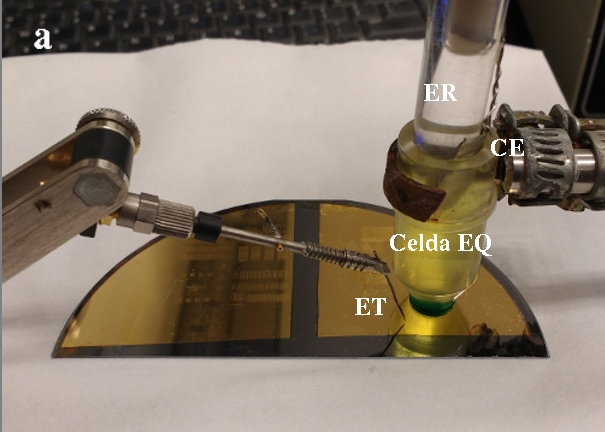
\includegraphics[width=\textwidth]{Imagenes/EQ1.jpg}
			  		  \end{subfigure}
			  		  \begin{subfigure}[t]{0.495\textwidth}
			  		  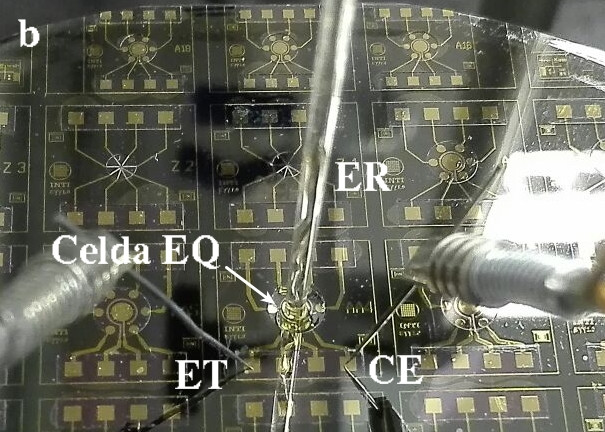
\includegraphics[width=\textwidth]{Imagenes/EQ2.jpg}
			  		  \end{subfigure}
			  \caption[Equipo para realizar la medidas electroquímicas]{Fotografía del instrumental que se utilizó a lo largo de la tesis para tomar las medidas electroquímicas. Izquierda: celda de acrílico sobre electrodos de Au recbierto con una \pdm\space utilizando CE y ER externos. Derecha: oblea con 6 ET por sensor, celda fabricada con resina epoxi SU8, CE integrado y utilizando un ER externo.}
			  		 \label{fig:celda}
			 		 \end{figure}	
					
			 		  
			Las mediciones electroquímicas fueron tomadas con un potencionestato \textit{Teq4}, para las medidas que se necesitaron velocidades de barrido mayores a \SI{1}{\volt\per\second} se utlizó un \textit{Autolab}, de la firma \textit{Ecochemie}. Como electrodo de referencia se empleó un electrodo saturado de calomel (ESC) de la firma \textit{Cole-Parmer} y como contraelectrodo (CE) se utilizaron indistintamente electrodos de Au depositados por pulverización catódica o una pieza de Pt de tamaño adecuado. En la tabla \ref{tabla:eq} se resumen los reactivos utilizados para llevar a cabo las mediciones electroquímicas. 
			
			A continuación se hace una breve reseña sobre las técnicas utilizadas, los parámetros empleados y las configuraciones experimentales.

			
				%Tabla ractivos EQ
				     \begin{table}[ht!]
			  		  \caption[Reactivos utilizados para las mediciones electroquímicas]{Reactivos y sondas electroquímicas utilizados para las mediciones electroquímicas}
			  		   \begin{tabular}{>{\raggedright\arraybackslash}m{4.4cm}>{\centering\arraybackslash}m{1.75cm}>{\centering\arraybackslash}m{2.7cm}>{\raggedright\arraybackslash}m{1.6cm}} 
			  		  \toprule
					  Reactivo \hspace{3cm}Nombre& Marca & Peso Molecular (\si{g.mol^{-1}}) & Función  \\ \midrule
			    	  \ferroCompleto \hspace{3cm} ferrocianuro de potasio & \textit{Sigma} & 422,41  & Sonda \\ \midrule
			    	  \ferriCompleto \hspace{3cm} ferricianuro de potasio & \textit{Sigma} & 329,27  & Sonda  \\ \midrule
			  		  \aminorutenioCompleto  \hspace{3cm}  cloruro de hexaaminorutenio& \textit{Aldrich} &  309,61  & Sonda  \\ \midrule
			  		  \raisebox{-.5\height}{\includegraphics[scale=0.4]{Esquemas/Fc.pdf}}  \hspace{3cm} ferroceno metanol   & \textit{Aldrich} &  216,06 & Sonda  \\ \midrule
			  		  H$_2$O \hspace{3cm} agua &  \SI{18}{\mega\ohm\per\cm}  &  18,02 & Solvente \\ \midrule
			  		  KCl  \hspace{3cm} cloruro de potasio   & \textit{Biopack} & 74,56 & Electrolito Soporte \\
 			  		  \bottomrule
			    	  \end{tabular}
			   		  \label{tabla:eq}
			   		  \end{table}
				   		  	
	 \subsection{Voltametría cíclica}
	 		
	 		La voltamperometría cíclica (VC) consiste en variar, de una manera cíclica, el potencial de un electrodo estacionario contra un electrodo de referencia. Ambos se encuentran inmersos en una solución en reposo y se mide la corriente resultante entre ellos. La señal de excitación es un barrido de potencial lineal con una onda de forma triangular, la cual parte de un potencial E$_1$, evoluciona linealmente hasta un potencial E$_2$ para luego volver a E$_1$. Las velocidades de este barrido pueden variar desde unos cuantos milivolts por segundo hasta cientos de volts por segundo; en nuestro caso se utilizaron velocidades próximas a los \SI{50}{\milli\volt.\second^{-1}}; se escogieron estas velocidades para llevar a cabo experimentos de una duración aceptable y que no se observe desplazamiento de potenciales para los picos de máxima oxidación y/o reducción, debido a limitaciones en la transferencia de carga por altas velocidades de barrido. \cite{nicholson1964,Gewirth2004}

	 		Como ya se dijo anteriormente se barre el potencial del electrodo de trabajo en dirección de ida y vuelta entre dos valores arbitrarios, E$_1$ y E$_2$. Al usar soluciones en base acuosa se debe trabajar en la región de estabilidad electroquímica del H$_2$O, para evitar reducción u oxidación de la misma, que genera H$_2$ u O$_2$ respectivamente. En la gran mayoría de los experimentos presentados en este trabajo se trabajó a un pH$\sim 5$, para el cual el rango de estabilidad del agua es entre \SI{-0.5}{\volt} y \SI{0.7}{\volt}, usando como referencia un electrodo saturado de calomel.\cite{wang2014} 

	 		En la figura \ref{fig:CV_ideal} se muestra la onda triangular de excitación aplicada y la curva obtenida para una sonda electroquímica idealmente reversible, donde se destacan los parámetros mas importantes.
	 		
	 		Esta técnica se utilizó para evaluar fenómenos de exclusión, permeación y preconcentración. También para determinar concentración de las sondas electroactivas dentro y fuera de los poros, calcular coeficientes de difusión y estimar distancias de sitios redox así como chequear accesibilidad y estructura de las películas delgadas mesoporosas.

	 			 \begin{figure}[ht]
			  		  \begin{subfigure}[t]{0.495\textwidth}
			  		  \includegraphics[width=\textwidth]{Graficos/onda-triangular.pdf}
			  		  \end{subfigure}
			  		  \begin{subfigure}[t]{0.495\textwidth}
			  		  \includegraphics[width=\textwidth]{Esquemas/CV-ideal.pdf}
			  		  \end{subfigure}
			  		  \caption[Voltamperometria ideal reversible]{Curva de excitación y voltagrama típico para una especie redox reversible.}
			  		  \label{fig:CV_ideal}
			  		  \end{figure}

	 		

	 \subsection{Voltametría cíclica de corriente alterna}

	 		La técnica de voltametría cíclica de corriente alterna (VCA) consta en aplicar una oscilación sinusoidal de voltaje a la celda electroquímica. A la onda triangular clásica usada en VC se la perturba, montando sobre ella, una pequeña onda de corriente alterna, en los experimentos presentados en este trabajo la perturbación fue de de \SI{10}{\milli\volt} y la frecuencia de la misma de 1 y \SI{2}{\hertz}. Esta técnica se emplea en conjunto con un analizador de frecuencias para filtrar la componente continua de la alterna, de este modo, ofrece un limite de detección menor e incrementa la sensibilidad respecto de la CV tradicional.\cite{Wi2000,Skoog1995}

	 		En la figura \ref{fig:ACV_ideal} se muestra la onda triangular con la perturbación, y la curva obtenida para una sonda electroquímica idealmente reversible, luego del filtrado de la componente continua.

	 		El propósito de esta técnica fue el obtener el coeficiente de difusión de hexaaminorutenio en sistemas porosos y contrastar con otras técnicas de forma de validar dicho coeficiente y los mecanismos de trasporte propuestos. 

	 			 \begin{figure}[hb]
			  		  \begin{subfigure}[t]{0.495\textwidth}
			  		  \includegraphics[width=\textwidth]{Graficos/onda-triangular-sin.pdf}
			  		  \end{subfigure}
			  		  \begin{subfigure}[t]{0.495\textwidth}
			  		  \includegraphics[width=\textwidth]{Graficos/ACV-ideal.pdf}
			  		  \end{subfigure}
			  		  \caption[Voltamperometria ideal reversible]{Curva de excitación y voltagrama típico para una especie redox reversible.}
			  		  \label{fig:ACV_ideal}
			  		  \end{figure}
	 		
	 		
			
	 \subsection{Simulaciones electroquímicas}\label{simulacion}

	 	 Con la finalidad de validar las hipótesis de transporte planteadas en el capitulo \ref{chap:Electroquimica} y establecer las condiciones en las que se pueden o no observar fenómenos de mediación electroquímica, se llevaron a cabo simulaciones numéricas de voltametrías cíclicas por computadora.

	 	 Se eligió realizar las simulaciones por el método de elementos finitos (MEF). El MEF es un método de calculo numérico, especialmente orientado a la resolución de ecuaciones diferenciales, de amplia difusión y para el cuál existen una gran cantidad programas con módulos preprogramados para diversas aplicaciones. En términos matemáticos, el MEF es una técnica numérica para la resolución de problemas descritos como un conjunto de ecuaciones diferenciales parciales. Comúnmente la ecuación básica que se necesita resolver para simular fenómenos electroquímicos es la ecuación de difusión, la cual relaciona la concentración $c$ con el tiempo $t$ y la distancia al electrodo $x$, dada por el coeficiente de difusión $D$.\cite{Britz2005,Nann2003} Esta ecuación se trata de un parábola de segundo orden en derivadas parciales y se la conoce como la segunda ley de Fick.\cite{fick1855}

	 	 \begin{equation}
	 	 	\frac{\partial c}{\partial t}=D\frac{\partial^2 c}{\partial^2 x}
	 	 	\label{eq:fick}
	 	 \end{equation}

	 	 Esta ecuación es la base del problema a la cual se le suman variables derivadas de las condiciones particulares de cada sistema que se quiera simular. 

	 	 %Convección, reacciones químicas, fenómenos de adsorción, y demás complicaciones son sólo algunos ejemplos que producen cambios en la concentración y en la difusión en sí. Para ellos se deben describir con precisión las condiciones de contorno particular para cada experimentos simulado.

	 	 El modelo aplicado en este trabajo utiliza condiciones de contorno de equilibrio (ecuación de Nerst) en la superficie del electrodo tanto para la sonda como para el mediador, lo cual es valido siempre que la cinética de electrodo sea suficientemente rápida. Dentro de la película mesoporosa se considera la difusión del mediador ($D$) y la sonda($D$) según la segunda ley de Fick (ecuación \ref{eq:fick}), utilizando coeficiente variables. En los caso en que se simuló una mediación redox, la reaccion entre entre ambos (sonda y mediador) fue descripta como una reaccion bimolecular de orden uno entre cada especie. En la solucion solo difunde la sonda. No se considera la migracion, lo cual es valido siempre y cuando la concentracion del electrolito soporte sea suficientemente alta. 

	     El modelo asume que el sistema es homogeneo en planos paralelos al electrodo y por lo tanto hay gradientes solo en la direccion normal al electrodo.   


	 	 Las simulaciones se se realizaron en colaboración con el Dr. Tagliasucchi del Instituto de Química Física de los Materiales, Medio Ambiente y Energía (INQUIMAE) con el software \textit{COMSOL Multiphysics\textsuperscript\textregistered} (\url{https://www.comsol.com/}) el cual simula las voltametrías utilizando elementos finitos. En la tabla \ref{tabla:simulacion} se resumen las variables utilizados para las simulaciones, sus valores y su descripción.
	 	
	    	\begin{table}[ht!]
	 	    \caption[Parámetros de las simulacinoes]{Parámetros y valores de entrada usadas durante las simulaciones de las voltametrías cíclicas.}
	 	    \begin{tabular}{>{\raggedright\arraybackslash}m{1.4cm}>{\centering\arraybackslash}m{2.8cm}>{\raggedright\arraybackslash}m{6.7cm}} 
	 	    \toprule
	 	    Variable  & 	Valor  &   descripción      \\ \midrule
	 	    $h$  	  &    \SI{200}{nm}	& 	   espesor de las películas delgadas mesoporosas 	    \\ \midrule
	 	    $C_{\fc}$  & \SI{5}{\milli\Molar}  & concentración de FeOH en solución    \\ \midrule
	 	    $C_{\ru}$ & \SI{1}{\milli\Molar}  & concentración de \ru\space en las películas    \\ \midrule
	 	    $k$ 		   & variable 	 & 	constante de mediación redox    \\ \midrule
	 	    $E^\circ_{\ru}$  & \SI{-0.3}{\volt} vs ESC & potencial reducción estandar el \ru \\ \midrule
	 	    $E^\circ_{\fc}$  & \SI{0.3}{\volt} vs ESC & potencial reducción estandar el \fc \\ \midrule
	 	    $D_{\fc}$  & variable & coeficiente de difusión del \fc\space en el film \\ \midrule
	 	    $D_{e}$  & variable & coeficiente de difusión por \textit{electron hopping }del \ru\space en el film \\ \midrule
	 	    $\nu$    & \SI{50}{\milli\volt\per\second}  &  velocidad de barrido \\
	 	     \bottomrule
			\end{tabular}
			\label{tabla:simulacion}
			\end{table} 

% Mail de mario
% Hola Gustavo,

% Recien miro lo que me enviaste. No se cuanto detalle queres agregar. Te mando un resumen breve...

% El metodo de elementos finitos es bastante estandar. Si queres leer un poco sobre su uso en electroquimica y citar algo de simulacion numerica, podes mirar el libro de Britz (Digital Simulation in Electrochemistry). Tiene muy poco sobre elementos finitos, pero creo que te alcanza. 

% El modelo usa condiciones de contorno de equilbrio (ecuacion de Nernst) en la superficie del electrodo tanto para la sonda como para el mediador, lo cual es valido siempre que la cinetica de electrodo sea rapida. Dentro del film se considera la difusion del mediador y la sonda (segunda ley de Fick) y ademas la reaccion redox entre ambos (reaccion bimolecular de orden uno entre cada especie). En la solucion solo difunde la sonda. No se considera la migracion, lo cual es valido siempre y cuando la concentracion del electrolito soporte sea suficientemente alta. 

% El modelo asume que el sistema es homogeneo en planos paralelos al electrodo y por lo tanto hay gradientes solo en la direccion normal al electrodo.   

% Decime si con eso te alcanza

% Saludos,

% Mario



%Revisión de LOGS

% B: /home/gustavo/Dropbox/Tesis/Capitulos/02_materiales.tex:56 Overfull --> tabla ok!
% B: /home/gustavo/Dropbox/Tesis/Capitulos/02_materiales.tex:57 Overfull --> tabla ok!
% B: /home/gustavo/Dropbox/Tesis/Capitulos/02_materiales.tex:58 Overfull --> tabla ok!
% B: /home/gustavo/Dropbox/Tesis/Capitulos/02_materiales.tex:268 Overfull --> tabla ok!
% B: /home/gustavo/Dropbox/Tesis/Capitulos/02_materiales.tex:268 Overfull --> tabla ok!
% B: /home/gustavo/Dropbox/Tesis/Capitulos/02_materiales.tex:269 Overfull --> tabla ok!
% B: /home/gustavo/Dropbox/Tesis/Capitulos/02_materiales.tex:270 Overfull --> tabla ok!
% B: /home/gustavo/Dropbox/Tesis/Capitulos/02_materiales.tex:270 Overfull --> tabla ok!
% B: /home/gustavo/Dropbox/Tesis/Capitulos/02_materiales.tex:271 Overfull --> tabla ok!
% B: /home/gustavo/Dropbox/Tesis/Capitulos/02_materiales.tex:275 Overfull --> tabla ok!
% B: /home/gustavo/Dropbox/Tesis/Capitulos/02_materiales.tex:0 Underfull --> Pagina de la foto de la alineadora, mucho espacio. Aceptable. OK!
% B: /home/gustavo/Dropbox/Tesis/Capitulos/02_materiales.tex:344 Overfull --> tabla ok!
% B: /home/gustavo/Dropbox/Tesis/Capitulos/02_materiales.tex:504 Overfull --> tabla ok!
% B: /home/gustavo/Dropbox/Tesis/Capitulos/02_materiales.tex:0 Underfull --> Pagina del esquema de la celda --> Aceptable 
% B: /home/gustavo/Dropbox/Tesis/Capitulos/02_materiales.tex:0 Underfull --> Pagina de la tabla de reactivos --> Aceptable
% B: /home/gustavo/Dropbox/Tesis/Capitulos/02_materiales.tex:556 Overfull --> tabla ok!